% Options for packages loaded elsewhere
\PassOptionsToPackage{unicode}{hyperref}
\PassOptionsToPackage{hyphens}{url}
%
\documentclass[
]{article}
\usepackage{amsmath,amssymb}
\usepackage{lmodern}
\usepackage{iftex}
\ifPDFTeX
  \usepackage[T1]{fontenc}
  \usepackage[utf8]{inputenc}
  \usepackage{textcomp} % provide euro and other symbols
\else % if luatex or xetex
  \usepackage{unicode-math}
  \defaultfontfeatures{Scale=MatchLowercase}
  \defaultfontfeatures[\rmfamily]{Ligatures=TeX,Scale=1}
\fi
% Use upquote if available, for straight quotes in verbatim environments
\IfFileExists{upquote.sty}{\usepackage{upquote}}{}
\IfFileExists{microtype.sty}{% use microtype if available
  \usepackage[]{microtype}
  \UseMicrotypeSet[protrusion]{basicmath} % disable protrusion for tt fonts
}{}
\makeatletter
\@ifundefined{KOMAClassName}{% if non-KOMA class
  \IfFileExists{parskip.sty}{%
    \usepackage{parskip}
  }{% else
    \setlength{\parindent}{0pt}
    \setlength{\parskip}{6pt plus 2pt minus 1pt}}
}{% if KOMA class
  \KOMAoptions{parskip=half}}
\makeatother
\usepackage{xcolor}
\usepackage[margin=1in]{geometry}
\usepackage{graphicx}
\makeatletter
\def\maxwidth{\ifdim\Gin@nat@width>\linewidth\linewidth\else\Gin@nat@width\fi}
\def\maxheight{\ifdim\Gin@nat@height>\textheight\textheight\else\Gin@nat@height\fi}
\makeatother
% Scale images if necessary, so that they will not overflow the page
% margins by default, and it is still possible to overwrite the defaults
% using explicit options in \includegraphics[width, height, ...]{}
\setkeys{Gin}{width=\maxwidth,height=\maxheight,keepaspectratio}
% Set default figure placement to htbp
\makeatletter
\def\fps@figure{htbp}
\makeatother
\setlength{\emergencystretch}{3em} % prevent overfull lines
\providecommand{\tightlist}{%
  \setlength{\itemsep}{0pt}\setlength{\parskip}{0pt}}
\setcounter{secnumdepth}{5}
\newlength{\cslhangindent}
\setlength{\cslhangindent}{1.5em}
\newlength{\csllabelwidth}
\setlength{\csllabelwidth}{3em}
\newlength{\cslentryspacingunit} % times entry-spacing
\setlength{\cslentryspacingunit}{\parskip}
\newenvironment{CSLReferences}[2] % #1 hanging-ident, #2 entry spacing
 {% don't indent paragraphs
  \setlength{\parindent}{0pt}
  % turn on hanging indent if param 1 is 1
  \ifodd #1
  \let\oldpar\par
  \def\par{\hangindent=\cslhangindent\oldpar}
  \fi
  % set entry spacing
  \setlength{\parskip}{#2\cslentryspacingunit}
 }%
 {}
\usepackage{calc}
\newcommand{\CSLBlock}[1]{#1\hfill\break}
\newcommand{\CSLLeftMargin}[1]{\parbox[t]{\csllabelwidth}{#1}}
\newcommand{\CSLRightInline}[1]{\parbox[t]{\linewidth - \csllabelwidth}{#1}\break}
\newcommand{\CSLIndent}[1]{\hspace{\cslhangindent}#1}
\ifLuaTeX
  \usepackage{selnolig}  % disable illegal ligatures
\fi
\IfFileExists{bookmark.sty}{\usepackage{bookmark}}{\usepackage{hyperref}}
\IfFileExists{xurl.sty}{\usepackage{xurl}}{} % add URL line breaks if available
\urlstyle{same} % disable monospaced font for URLs
\hypersetup{
  pdftitle={Evaluating Clustering Techniques on Non-elliptical Data},
  pdfauthor={Safiya Sirota, Yijin Wang, Bin Yang},
  hidelinks,
  pdfcreator={LaTeX via pandoc}}

\title{Evaluating Clustering Techniques on Non-elliptical Data}
\author{Safiya Sirota, Yijin Wang, Bin Yang}
\date{}

\begin{document}
\maketitle

{
\setcounter{tocdepth}{2}
\tableofcontents
}
\hypertarget{background-and-objective}{%
\section{Background and Objective}\label{background-and-objective}}

Latent Class Analysis and K-means are two successful clustering
algorithms that partition the given data into distinct subgroups where
observations in each group are very similar. They are popular choice of
method in solving healthcare research problems such as identifying
clusters on microscopic images (Amin et al. 2015), categorizing suicides
by risk factors (Logan, Hall, and Karch 2011), and grouping elderly
patients with their access to health care (Thorpe et al. 2011). One
important assumption that both of these algorithms require is the
normality of the given data.

In our project, we focus on the unsupervised learning scenario and we
investigate how well these two algorithms perform when the normality
assumption is violated. We designed 4 simulation settings as violation
of the normality assumption: 1) skewed data, 2) data with heavy tail, 3)
data with outliers, 4) multimodal data. In the end, we compare their
performance with Rand Index in each settings with varying sample sizes.

\hypertarget{statistical-method}{%
\section{Statistical Method}\label{statistical-method}}

\hypertarget{k-means}{%
\subsection{K Means}\label{k-means}}

K-means clustering is a popular clustering algorithm that partitions
data into a prespecified number of clusters. The goal for k-means is to
find clusters such that the total within-cluster variation is minimized.
Formally, the within-cluster variation is defined as follows:

\[tot.withinss = \sum_{i=1}^kW(C_k) = \sum_{i=1}^k\sum_{x\in c_k}(x_i-\mu_k)^2\]

A general procedure of the k-means algorithm can be described as
follows:\\
(1) Specify number of clusters \(k\).\\
(2) Assign each observation to their closest centroid, minimizing
\(W(C_k)\).\\
(3) For each cluster, update the cluster centroid by calculating the new
mean values of all the data points in the cluster. The centroid of a
\(K_{th}\) cluster is a vector of length \(p\) containing the means of
all variables.\\
(4) Iteratively minimize the total within sum of square. That is,
iterate steps 3 and 4 until the cluster assignments stop changing or the
maximum number of iterations is reached.

Specifying the number of clusters is a crucial step for the K means
algorithms. There are multiple ways to determine the optimal number of
clusters for k-means. In this project, we use the average silhouette
method, which provides a measure of the similarity of an object is to
its own cluster compared to other clusters. This method chooses the
optimal number of clusters \(k\) that maximized the average silhouette.

\hypertarget{latent-class-analysis}{%
\subsection{Latent Class Analysis}\label{latent-class-analysis}}

In contrast to K means algorithm which uses a distance based criteria,
LCA is a model-based clustering approach that derives clusters using a
Gaussian finite mixture modeling that describes distribution the data.
We use the R package \(\textbf{mclust}\) for this task which allows a
wide range of parameterizations of the data as shown in figure 1(Scrucca
et al. 2016).

\begin{figure}
\centering
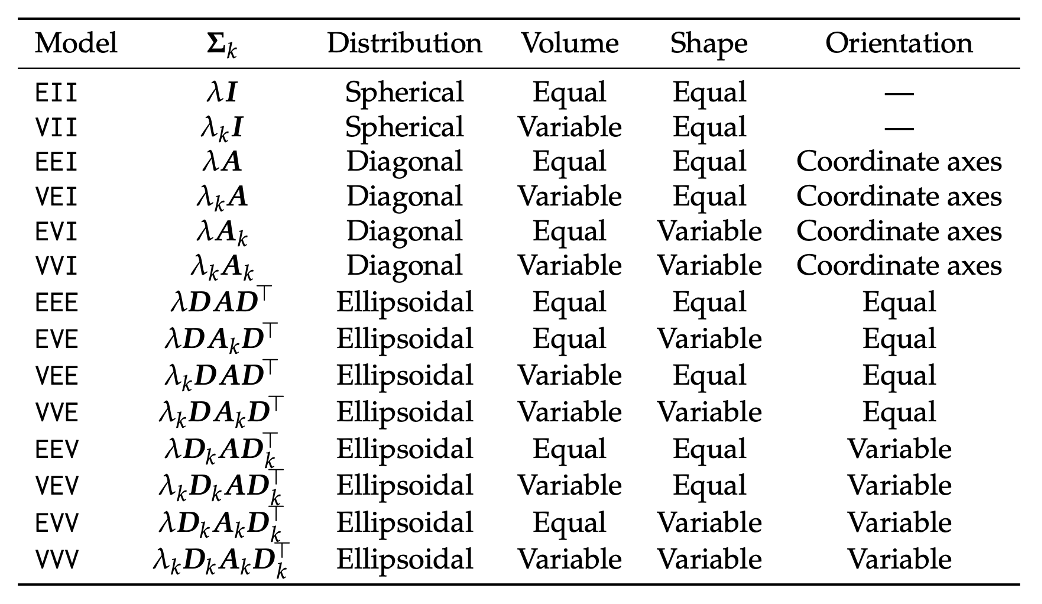
\includegraphics[width=4.16667in,height=\textheight]{report_image/mclust_table}
\caption{Parameterisations of the within-group covariance matrix for
multidimensional data available in the mclust package, and the
corresponding geometric characteristics.}
\end{figure}

LCA uses finite mixture modeling for parameter estimation, which is
crucial to determining the number of components. A variety of approaches
can be used to estimate the component number and in this project, we
utilize the Bayesian Information Criterion (BIC) for this task. BIC is
one of the popular choice for model selection in the context of Gaussian
Mixture Modeling. It takes on a penalized forms of the log-likelihood
where a penalty term for the number of estimated parameters is
subtracted from the log-likelihood. Formally,
\[BIC_{M,G} = 2l_{M,g}(X|\hat{\Psi}) - v\text{log}(n)\] where
\(l_{M,g}(X|\hat{\Psi})\) is the log-likelihood at the MLE
\(\hat{\Psi}\) for model \(M\) with \(G\) components, \(n\) is the
sample size, and \(v\) is the number of estimated parameters The pair
\({M, G}\) which maximizes \(BIC_{M,G}\) is selected as the final model.

\hypertarget{performance-metric}{%
\section{Performance Metric}\label{performance-metric}}

We use the Rand index as our performance metric in this study. It is
used to compare the similarity of results between two different
clustering methods. In our case, we compare our k-means or LCA
clustering results to the true clustering that we have defined through
our data generation.

Given a set of \(n\) elements \(S = \{o_1, \dots, o_n\}\) and two
partitions of S to compare, \(X = \{X_1, \dots, X_r\}\), and
\(Y = \{Y_1, \dots, Y_s\}\) we denote \(a\) as the number of times a
pair of elements belongs to the same cluster across two clustering
methods. And we denote \(b\) as the number of times a pair of elements
belong to different clusters across the two methods. Finally, the Rand
index is

\begin{equation*}
R = \frac{a+b}{{2 \choose n}},
\end{equation*}

which measures the proportion of agreement of two clustering methods in
all unordered pairs.

\hypertarget{simulations-settings-and-results}{%
\section{Simulations Settings and
Results}\label{simulations-settings-and-results}}

In simulations, we consider bivariate data with 2 true clusters. We
generated data from different non-elliptical distributions in each
setting.

For each simulation setting, we create 100 runs using randomly generated
data sets in size of 500, 1000, 5000 and evaluate the Rand index for
each method.

\hypertarget{skewed-data}{%
\subsection{Skewed Data}\label{skewed-data}}

\hypertarget{data-generation}{%
\subsubsection{Data Generation}\label{data-generation}}

In this setting, we want to test the performance of K-means and LCA when
all features follow a skewed distribution. We assume the features
\(X_1, X_2\) are independent.

All data in the first feature \(X_{11}, X_{12},..X_{1N}\) are random
draws from a mixture model of Weibull distributions with density
\(0.5f_1(x|1,5) + 0.5f_2(x|12,14)\) where \(f_1 \sim Weibull(1,5)\) and
\(f_2 \sim Weibull (12,14)\).

Similarly, all data in the second feature \(X_{21}, X_{22},..X_{2N}\)
are random draws from another mixture model of Weilbull distributions
with density \(0.5f_3(x|1,3) + 0.5f_4(x|1,4)\) where
\(f_3 \sim Weibull(1,3)\) and \(f_4 \sim Weibull (1,4)\).

We generate 2 equal-sized clusters with total size being 500, 1000 and
5000. An example of a sample with size 5000 is shown below.

\begin{figure}
\centering
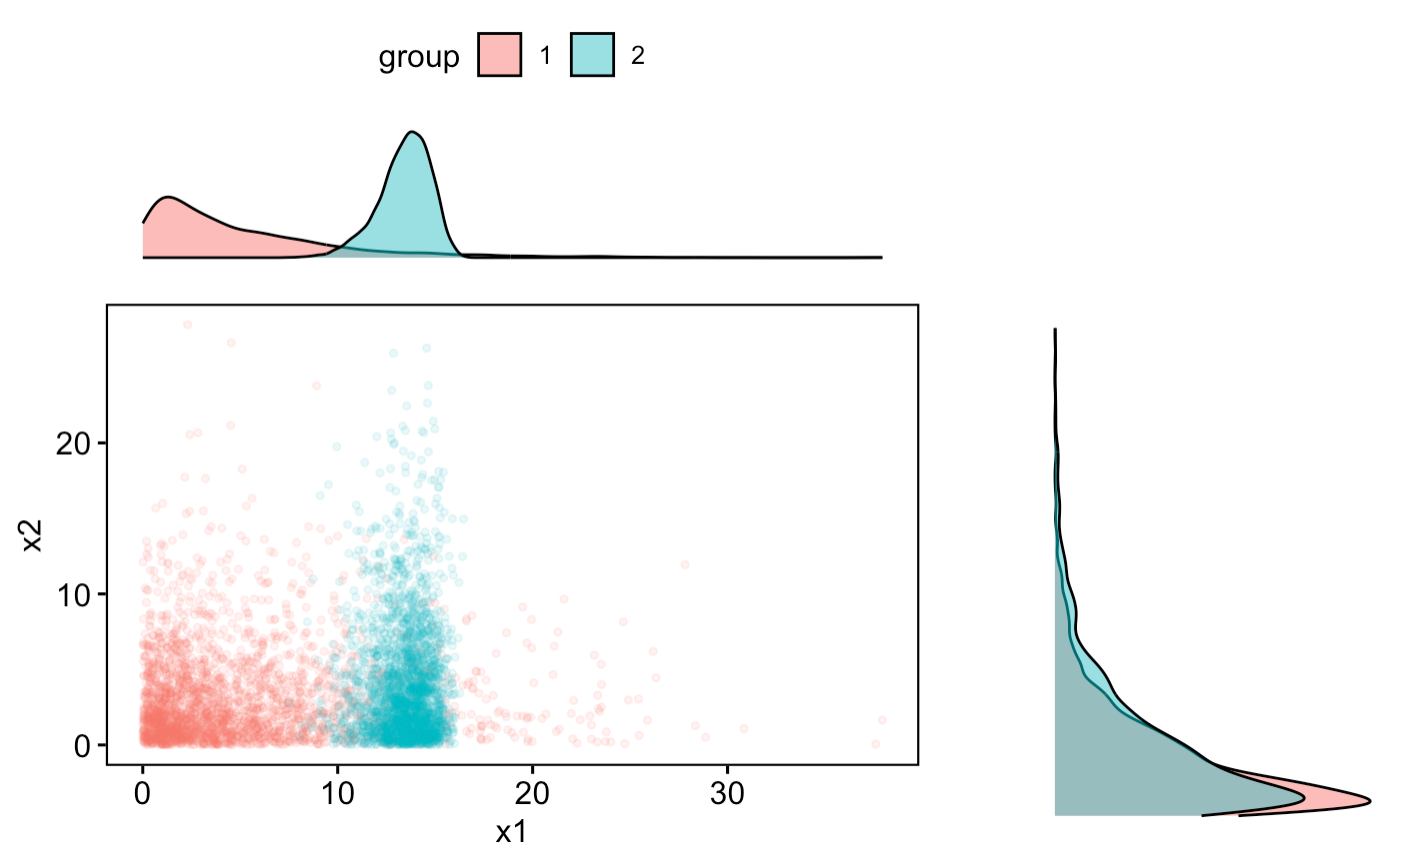
\includegraphics[width=4.16667in,height=\textheight]{report_image/skewed_sample.png}
\caption{Skewed Data Sample}
\end{figure}

\hypertarget{results}{%
\subsubsection{Results}\label{results}}

We are interested in how well K-means and LCA perform when the input
data already has two true clusters. We calculate Rand Index for sample
data in each simulation run and conclude that after 100 simulations,
K-means performs better than LCA across all sample sizes. As sample size
increases, the variance of Rand Index decreases.

\begin{figure}
\centering
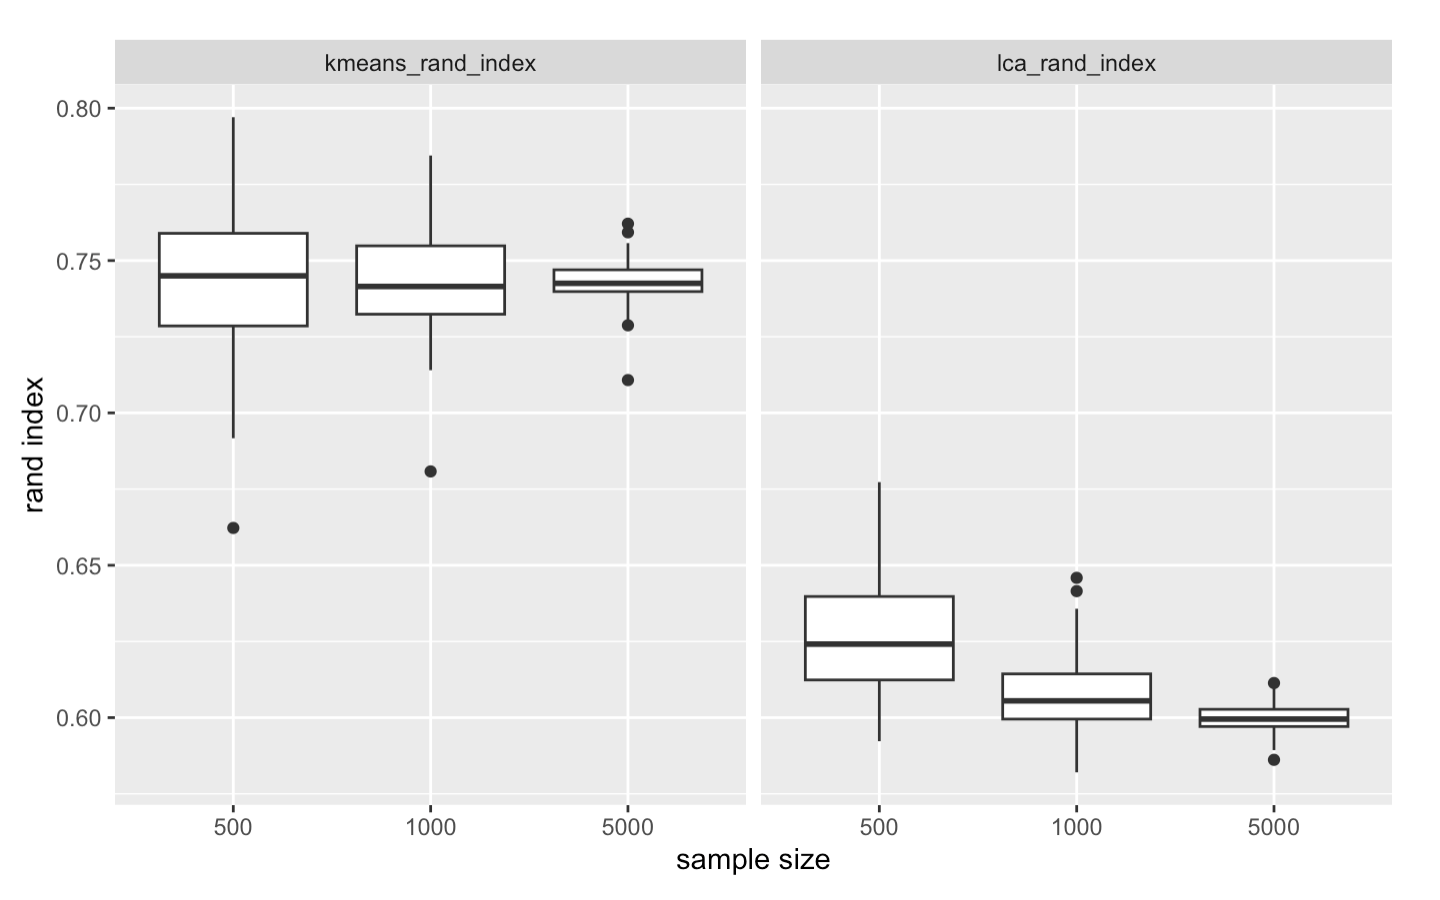
\includegraphics[width=4.16667in,height=\textheight]{report_image/skewed_data_rand_index_results.png}
\caption{Skewed Data Comparison - Rand Index}
\end{figure}

To investigate some potential reasons behind this, we compare the
optimal number of cluster number for each method in all simulations.
Choosing the optimal cluster number is the first step for both methods.
This number is crucial to our comparison because we predetermined the
number of true clusters to be 2 and Rand Index uses the number of
agreements in its calculation. Therefore, having a cluster number that
is larger than 2 could hurt the performance.

In this figure, we compare the optimal number of clusters. Overall,
K-means choose its optimal number of cluster around 3 which is much
lower than that of LCA across all sample sizes. As sample size
increases, the optimal number of cluster increases for LCA as well.

\begin{figure}

{\centering 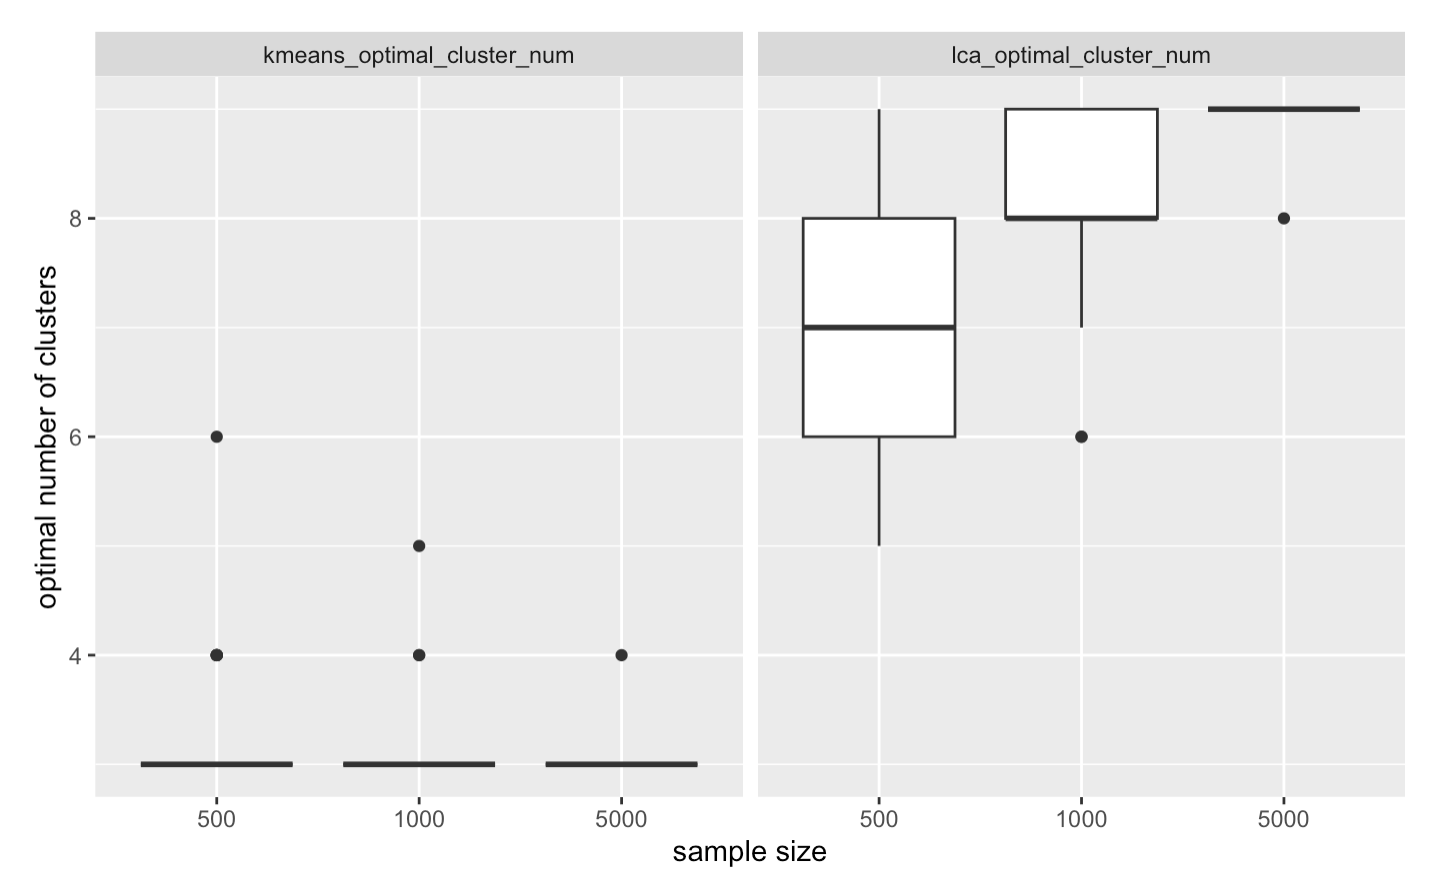
\includegraphics[width=0.5\linewidth]{report_image/skewed_data_num_clusters_results} 

}

\caption{Skewed Data Comparison - Optimal Number of Clusters}\label{fig:unnamed-chunk-1}
\end{figure}

\hypertarget{multimodal-data}{%
\subsection{Multimodal Data}\label{multimodal-data}}

\hypertarget{data-generation-1}{%
\subsubsection{Data Generation}\label{data-generation-1}}

In this setting, we have two independent variables \(X\) and \(Y\),
which both follow the same bimodal mixture distribution. Variables \(X\)
and \(Y\) can each be partitioned into two parts, \(\{X_1, X_2\}\) and
\(\{Y_1, Y_2\}\), where \(X_1\), \(Y_1\) are drawn from one bimodal
distribution and \(X_2\), \(Y_2\) are drawn from a different bimodal
distribution, as specified below.

\begin{align*}
  X_1, Y_1 & \sim 
  \begin{cases}
    N(-3, \frac{3}{4}) & w/\ prob.\ 0.5 \\
    N(0, \frac{3}{4}) & w/\ prob.\ 0.5
  \end{cases} \\
  X_2, Y_2 & \sim
  \begin{cases}
    N(3, \frac{3}{4}) & w/\ prob.\ 0.5 \\
    N(6, \frac{3}{4}) & w/\ prob.\ 0.5
  \end{cases}
\end{align*}

Since each bimodal distribution is a mixture of two Gaussian
distributions, these data follow a Gaussian mixture distribution,
leading to four distinct latent clusters. This can be seen in the figure
below, which graphs an example dataset on X and Y axes and colors the
data points by cluster.

\begin{figure}
\centering
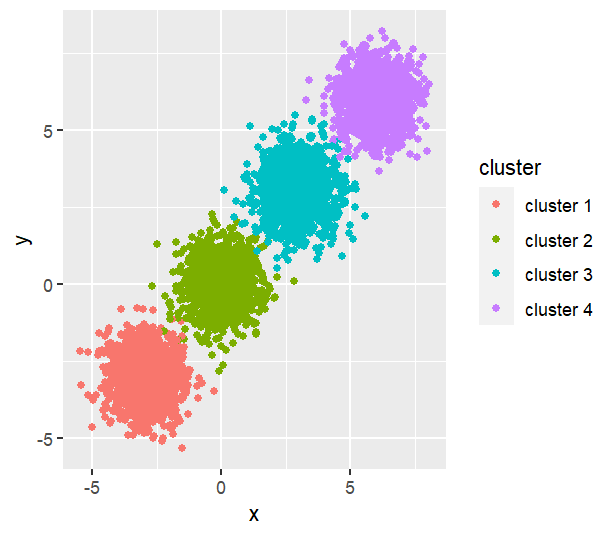
\includegraphics{report_image/multimodal_clusters.png}
\caption{Mutlimodal Data - Latent Clusters}
\end{figure}

Since this is a mixture Gaussian case, we should expect LCA to perform
very well since it assumes mixture Gaussian data. K-mean should also
perform well, since k-means is proven to identify cluster in normal data
well.

\hypertarget{results-1}{%
\subsubsection{Results}\label{results-1}}

We found that the median Rand index for 100 runs using k-means with
sample size \(n=500\) was 0.99 (IQR: 0.17) while for LCA it was 1 (IQR:
0). For sample size was \(n=1000\) the median Rand index for k-means was
0.99 (IQR: 0.25) and for LCA it was 1 (IQR: 0). For sample size
\(n=5000\) the median Rand index for k-means was 1 (IQR: 0) and it was
the same for LCA. These results are visualized below and show that
k-means and LCA both perform almost perfectly in this case, with LCA
performing better when the sample size is smaller. Variation from a Rand
index of 1 (i.e., perfect classification) comes in only when k-means or
LCA algorithms do not choose the correct number of clusters initially.

\begin{figure}
\centering
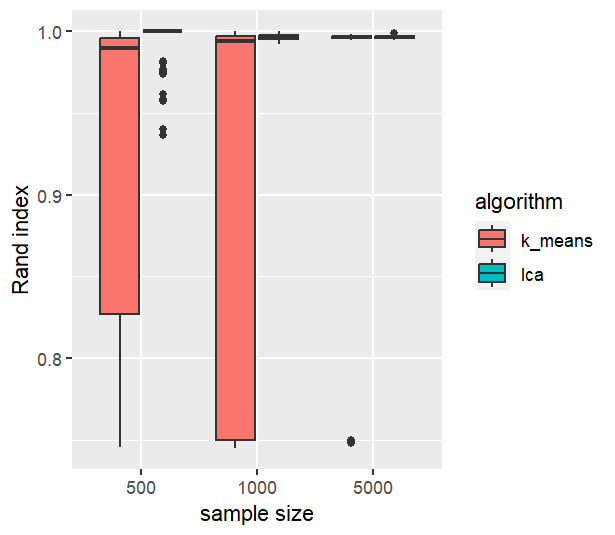
\includegraphics{report_image/multimodal_results.png}
\caption{Mutlimodal Data - Results}
\end{figure}

\hypertarget{heavy-tails-data}{%
\subsection{Heavy Tails Data}\label{heavy-tails-data}}

\hypertarget{data-generation-2}{%
\subsubsection{Data Generation}\label{data-generation-2}}

To investigate the algorithm performance in the heavy tails data
setting, we consider generating data from a mixture of the Cauchy
distribution with two latent clusters. Specifically, we sample
\(X_{1i}, i = 1...N\) from a mixture of Cauchy distribution
\(\lambda_1f_1 + \lambda_2f_2\) where
\(f_1 \sim \text{Cauchy}(-3,3), f_2 \sim \text{Cauchy}(3,0.5)\) and we
set the mixing weights \(\lambda_1 = \lambda_2 = 0.5\) corresponding to
the latent cluster \(1,2\). We further sample \(X_{2i}\) from an
independent Gaussian distribution \(\text{N}(0,1)\).

We first examine the generated data via scatter plot and the density
plot where the two colors denote two latent clusters. By a direct
observation of these plots, we notice the two latent clusters are not
easily separated.

\begin{figure}

{\centering 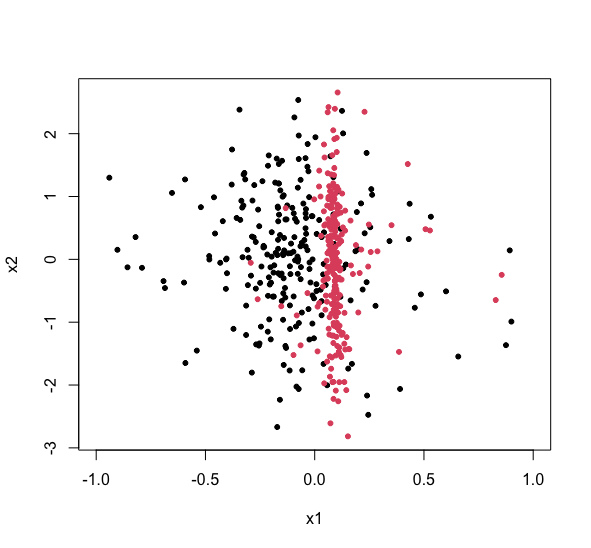
\includegraphics[width=0.49\linewidth]{report_image/cauchy} 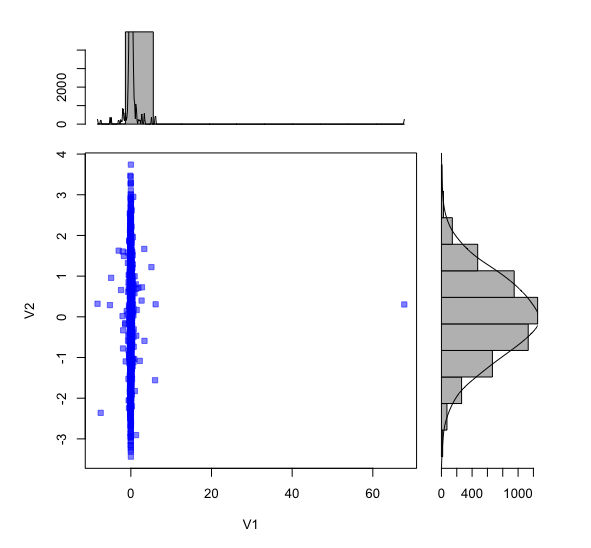
\includegraphics[width=0.49\linewidth]{report_image/cauchy_2} 

}

\caption{Scatter and density plot for the mixture of Cauchy distribution}\label{fig:unnamed-chunk-2}
\end{figure}

\hypertarget{results-2}{%
\subsubsection{Results}\label{results-2}}

We examine the model performance of K means and LCA via 100 runs of
simulation with sample sizes \(N = 500, 1000, 5000\) using Rand index.
We observe that in all our simulation settings, LCA performed better
than K means in terms of Rand index. As sample size increases, LCA
performed worse.

\begin{figure}

{\centering 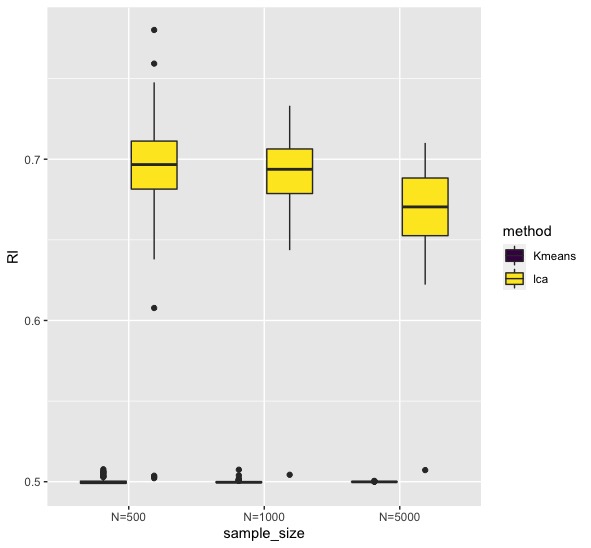
\includegraphics[width=0.5\linewidth]{report_image/RI_cauchy} 

}

\caption{Boxplot of Rand Index for the mixture of Cauchy distribution }\label{fig:unnamed-chunk-3}
\end{figure}

\hypertarget{prsence-of-outliers}{%
\subsection{Prsence of Outliers}\label{prsence-of-outliers}}

\hypertarget{data-generation-3}{%
\subsubsection{Data Generation}\label{data-generation-3}}

Finally, we investigate the scenario where there exits outliers in the
data. We first generate \(X_{1i}, i = 1,...,N\) from a mixture of
Gaussian distribution \(\lambda_1f_1 + \lambda_2f_2\) where
\(f_1 \sim \text{N}(0,1), f_2 \sim \text{N}(3,1)\) and we set the mixing
weights \(\lambda_1 = \lambda_2 = 0.5\) corresponding to the latent
cluster \(1,2\). We further sample \(X_{2i}\) from an independent
Gaussian distribution \(\text{N}(0,1)\). We then generate outliers
\(\epsilon\) from \(\text{N}(30,1), \text{N}(-30,1)\) and \(\epsilon's\)
are added to \(X_1\) with equal probabilities of \(0.05\) generated from
\(\text{bernouli}(0.05)\).

Similarly, we examine examine the generated data via scatter plot and
the density plot where the two colors denote two latent clusters.

\begin{figure}

{\centering 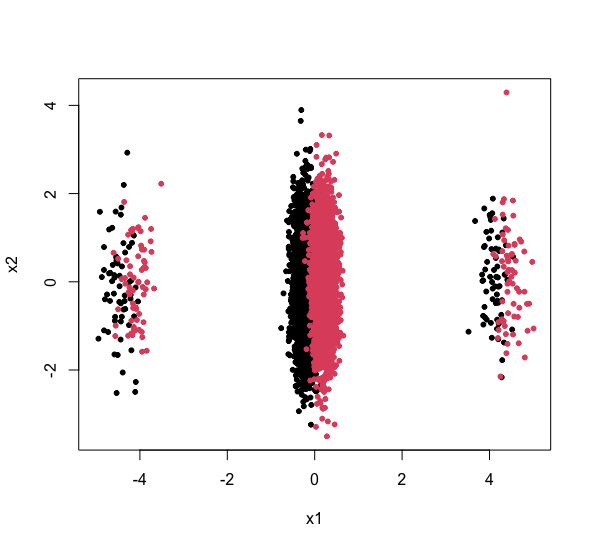
\includegraphics[width=0.49\linewidth]{report_image/outlier} 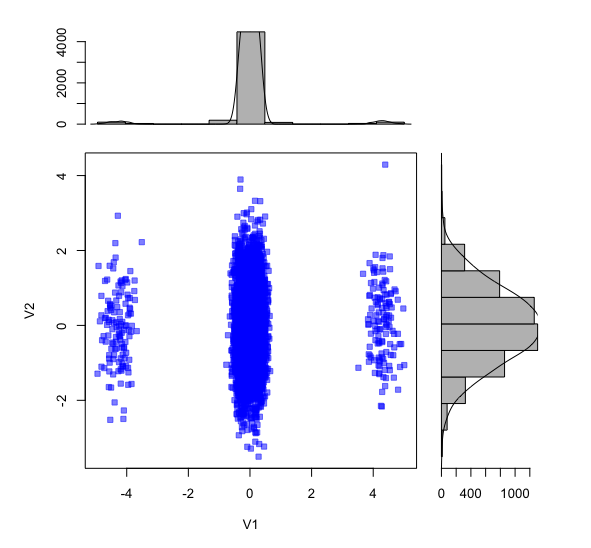
\includegraphics[width=0.49\linewidth]{report_image/outlier2} 

}

\caption{Scatter and density plot for data with Gaussian outlier}\label{fig:unnamed-chunk-4}
\end{figure}

\hypertarget{results-3}{%
\subsubsection{Results}\label{results-3}}

Similarly, performance of K means and LCA via is examinined 100 runs of
simulation with sample sizes \(N = 500, 1000, 5000\) using Rand index.
We observe that in all our simulation settings, LCA performed better
than K means in terms of Rand index.

\begin{figure}

{\centering 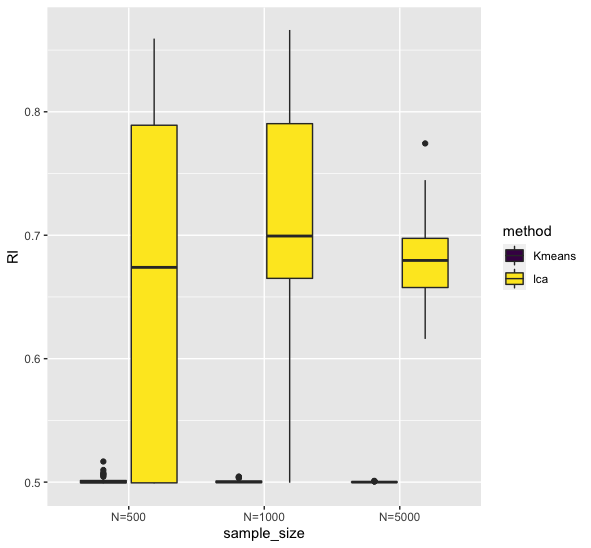
\includegraphics[width=0.5\linewidth]{report_image/RI_outlier} 

}

\caption{Boxplot of Rand Index for data with Gaussian outlier }\label{fig:unnamed-chunk-5}
\end{figure}

\hypertarget{discussion}{%
\section{Discussion}\label{discussion}}

\hypertarget{conclusion}{%
\subsection{Conclusion}\label{conclusion}}

In conclusion, we found that for skewed data, k-means performs better
than LCA. However, in all other cases, LCA outperformed k-means, except
in the case where the data follows a Gaussian mixture distribution and
the sample size of the dataset is very large, in which case k-means and
LCA perform similarly.

\hypertarget{limitations}{%
\subsection{Limitations}\label{limitations}}

In this study, we found that there is no uniformly best algorithm for
identifying latent clusters in data. This leads us to believe that
knowing how the data is generated is important for deciding whether to
use k-means or LCA. However, this information is rarely known.

We also found that variation in correct classification for both
algorithms often comes from choosing the number of clusters. There are
many ways to choose the number of clusters before actually performing
the clustering algorithm. Varying these methods goes beyond the scope of
this study, but future research should test k-means against LCA under
different cluster number selection techniques.

In summation, we suggest that researchers make informed speculations
about the shape and potential number of latent clusters in their data
before running either k-means or LCA in order to get the best results.

\hypertarget{references}{%
\section{References}\label{references}}

\hypertarget{refs}{}
\begin{CSLReferences}{1}{0}
\leavevmode\vadjust pre{\hypertarget{ref-amin_recognition_2015}{}}%
Amin, Morteza Moradi, Saeed Kermani, Ardeshir Talebi, and Mostafa
Ghelich Oghli. 2015. {``Recognition of {Acute} {Lymphoblastic}
{Leukemia} {Cells} in {Microscopic} {Images} {Using} {K}-{Means}
{Clustering} and {Support} {Vector} {Machine} {Classifier}.''}
\emph{Journal of Medical Signals and Sensors} 5 (1): 49--58.
\url{https://www.ncbi.nlm.nih.gov/pmc/articles/PMC4335145/}.

\leavevmode\vadjust pre{\hypertarget{ref-logan_suicide_2011}{}}%
Logan, Joseph, Jeffrey Hall, and Debra Karch. 2011. {``Suicide
{Categories} by {Patterns} of {Known} {Risk} {Factors}: {A} {Latent}
{Class} {Analysis}.''} \emph{Archives of General Psychiatry} 68 (9):
935--41. \url{https://doi.org/10.1001/archgenpsychiatry.2011.85}.

\leavevmode\vadjust pre{\hypertarget{ref-scrucca2016mclust}{}}%
Scrucca, Luca, Michael Fop, T Brendan Murphy, and Adrian E Raftery.
2016. {``Mclust 5: Clustering, Classification and Density Estimation
Using Gaussian Finite Mixture Models.''} \emph{The R Journal} 8 (1):
289.

\leavevmode\vadjust pre{\hypertarget{ref-thorpe_patterns_2011}{}}%
Thorpe, Joshua M., Carolyn T. Thorpe, Korey A. Kennelty, and Nancy
Pandhi. 2011. {``Patterns of Perceived Barriers to Medical Care in Older
Adults: A Latent Class Analysis.''} \emph{BMC Health Services Research}
11 (1): 181. \url{https://doi.org/10.1186/1472-6963-11-181}.

\end{CSLReferences}

\end{document}
